\documentclass[a4paper,12pt]{article}

%%% Работа с русским языком
\usepackage{cmap}					% поиск в PDF
\usepackage{mathtext} 				% русские буквы в формулах
\usepackage[T2A]{fontenc}			% кодировка
\usepackage[utf8]{inputenc}			% кодировка исходного текста
\usepackage[english,russian]{babel}	% локализация и переносы
\usepackage{xcolor}
\usepackage{hyperref}
 % Цвета для гиперссылок
\definecolor{linkcolor}{HTML}{799B03} % цвет ссылок
\definecolor{urlcolor}{HTML}{799B03} % цвет гиперссылок

\hypersetup{pdfstartview=FitH,  linkcolor=linkcolor,urlcolor=urlcolor, colorlinks=true}

%%% Дополнительная работа с математикой
\usepackage{amsfonts,amssymb,amsthm,mathtools} % AMS
\usepackage{amsmath}
\usepackage{icomma} % "Умная" запятая: $0,2$ --- число, $0, 2$ --- перечисление

%% Номера формул
%\mathtoolsset{showonlyrefs=true} % Показывать номера только у тех формул, на которые есть \eqref{} в тексте.

%% Шрифты
\usepackage{euscript}	 % Шрифт Евклид
\usepackage{mathrsfs} % Красивый матшрифт

%% Свои команды
\DeclareMathOperator{\sgn}{\mathop{sgn}}

\newcommand*{\hm}[1]{#1\nobreak\discretionary{}
{\hbox{$\mathsurround=0pt #1$}}{}}
% графика
\usepackage{graphicx}
\graphicspath{{pictures/}}
\DeclareGraphicsExtensions{.pdf,.png,.jpg}
\author{Бурмашев Григорий}
\title{Матан, коллок - 1 }
\date{\today}
\begin{document}
\begin{center}
Бурмашев Григорий. 208. Дискра - 5
\end{center}
\section*{Номер 1}
Пусть в дереве есть 2 вершины: a и b. Тогда для одного ребра есть два возможных варианта циклов длины 2:
\[
(aba)
\]
\[
(bab)
\]
В дереве на 12 вершинах $n - 1 = 12 - 1 = 11 $ ребер. Каждое ребро дает нам 2 цикла, а значит всего  $11 \cdot 2 = 22$ цикла.
\begin{center}
\textbf{Ответ:} 22 цикла
\end{center}

\section*{Номер 2}
Пусть у нас есть две вершины степени 5: a и b. Максимум одно из пяти ребер, выходящих из a, ведет в b. И еще 4 ребра из b ведут в другие вершины. Итого 9 ребер. Но в дереве на 9 вершинах $9 - 1 = 8 $ ребер. Мы видим \textbf{противоречие} $ \rightarrow$ это невозможно
\begin{center}
\textbf{Ответ:} нет
\end{center}

\section*{Номер 3}
Т.к это связный граф, то максимальное количество вершин будет, если граф будет иметь вид <<цепочки>> из вершин степени 2, за исключеним двух вершин, которые являются началом и концом этой цепочки и имеют степени 1. Тогда у нас останется $20 - 1 - 1 = 18 $ степеней вершин, а значит вершин степени 2 у нас: $\frac{18}{2} = 9$. Всего, в таком случае, 9 + 2 = 11 вершин. Взять больше вершин степени 1 нельзя, т.к тогда граф перестанет быть связным.
\begin{center}
\textbf{Ответ:} 11 вершин.
\end{center}

\section*{Номер 4}
Можно привести пример дерева на 2020 вершинах, в котором нет простого пути длины 3, а именно:

Это дерево с вершиной u степени 2019, из которой выходят ребра в 2019 вершин степени 1. Мы получаем дерево на 2020 вершинах, в котором максимальный простой путь длины 2, т.е: 
\begin{center}
(любая из 2019 вершин степени 1 - u - любая из оставшихся 2018 вершин)
\end{center}
\begin{center}
\textbf{Ответ:} нет
\end{center}
\begin{center}
Изображение:
\end{center}
\begin{center}
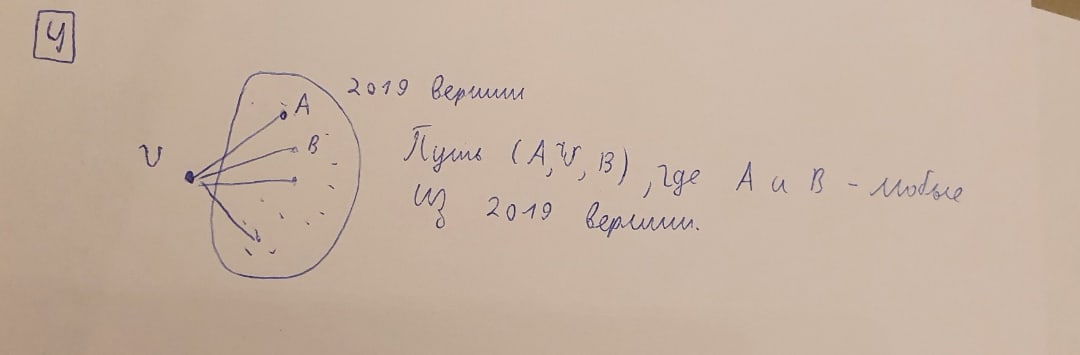
\includegraphics[scale=0.4]{4.jpg}
\end{center}

\section*{Номер 5}
В связном графе наименьшее количество ребер будет, если граф -- дерево. Но в условии сказано, что в графе нет мостов. Тогда наш граф -- цикл из n вершин степени 2. При удалении любой из вершин количество компонент связности не изменится, а ребер в нем всего $n -1 + 1 = n$ (n-1 ребро в дереве + 1 ребро, образующее цикл)

\begin{center}
\textbf{Ответ:} n ребер
\end{center}
\section*{Номер 6}
От обратного:

Пусть есть ребро, которое является мостом для множеств вершин A и B в графе и соединяет две вершины a и b. Удалим его. Тогда мы получим две компонентны связности (A и B) Тогда степени вершин a и b будут нечетными (четное - 1 = нечетное), при этом у оставшихся вершин степени все еще остаются четными. А значит сумма степеней вершин как в A, так и в B будет нечетной. Но мы знаем, что сумма степеней внутри одной компоненты связности всегда четна, т.е мы получили \textbf{противоречие} и моста в таком графе нет.
\begin{center}
\textbf{Ч.Т.Д}
\end{center}
\section*{Номер 7}
Построим граф на 6ти вершинах A. Либо в самом графе, либо в дополнении есть как минимум 3 ребра.  Пусть в графе у нас есть ребра (ab), (ac) и (ad). Если у нас есть хотя бы одно из ребер (bc), (cd) или (bd), то мы получаем хотя бы один цикл длины 3: либо (abc), либо (acd), либо (abd) и граф соотвествует утверждению. Пусть тогда нет ни одного из ребер (bc), (cd) и (bd), но в таком случае мы точно знаем, что они есть в дополнении графа  А  $\rightarrow$ там есть хотя бы один цикл длины 3.

Аналогично при изначальном рассмотрении дополнения графа. Т.е при отсутствии там ребер (bc), (cd) и (bd) циклы длины 3 образуются в графе A.

А значит в любом графе на 6 и более вершинах у нас есть хотя бы один цикл длины 3 
\begin{center}
\textbf{Ч.Т.Д}
\end{center}
\begin{center}
Изображение:
\end{center}
\begin{center}

\includegraphics[scale=0.2]{8.jpg}
\end{center}
\section*{Номер 9}
Зафиксируем одну висячую вершину. Т.к в нашем дереве нет вершин степени 2, то из это висячей вершины выходит одна вершина степени как минимум 3, из которой выходят еще как минимум 2 вершины и так далее... Пусть <<снизу>> у нас x висячих вершин и еще 1 в самом начале графа. Тогда всего $ x + 1 $  висячая вершина. В таком случае вершин степени 3 и выше:
\[
\frac{x}{2}  + \frac{x}{4} + \frac{x}{8} + \ldots
\]
Т.к в каждую из x вершин можно попасть как минимум из двух вершин. Т.е поднимаясь снизу вверх по графу мы как минимум удваиваем кол-во вершин на каждом уровне.
\[
\frac{x}{2}  + \frac{x}{4} + \frac{x}{8} + \ldots \leq x \leq x + 1
\]
При максимальном числе вершин всего у нас $x + 1 + x$ вершин. При этом:
\[
\frac{2x+1}{2} \leq x + 1
\]
\[
2x + 1 \leq 2x + 2
\]
\[
1 \leq 2
\]
Т.е число висячих вершин больше или равно половине общего числа вершин.
\begin{center}
\textbf{Ч.Т.Д}
\end{center}

\end{document}